
%% General definitions
\documentclass{article} %% Determines the general format.
\usepackage{a4wide} %% paper size: A4.
\usepackage[utf8]{inputenc} %% This file is written in UTF-8.
%% Some editors on Windows cannot save files in UTF-8.
%% If there is a problem with special characters not showing up
%% correctly, try switching "utf8" to "latin1" (ISO 8859-1).
\usepackage[T1]{fontenc} %% Format of hte resulting PDF file.
\usepackage{fancyhdr} %% Package to create a header on each page.
\usepackage{lastpage} %% Used for "Page X of Y" in the header.
											%% For this to work, you have to call pdflatex twice.
\usepackage{enumerate} %% Used to change the style of enumerations (see below).

\usepackage{amssymb} %% Definitions for math symbols.
\usepackage{amsmath} %% Definitions for math symbols.
\usepackage{amsthm}
\usepackage{braket}
\usepackage{graphicx}
\usepackage{float}
\usepackage{hyperref}

\usepackage{tikz}  %% Pagacke to create graphics (graphs, automata, etc.)
\usetikzlibrary{automata} %% Tikz library to draw automata
\usetikzlibrary{arrows}   %% Tikz library for nicer arrow heads


%% Left side of header
\lhead{\course\\\semester\\Exercise \homeworkNumber}
%% Right side of header
\rhead{\authorname\\Page \thepage\ of \pageref{LastPage}}
%% Height of Header
\usepackage[headheight=36pt]{geometry}
%% Page style that uses the header
\pagestyle{fancy}

\newcommand{\authorname}{Nico Bachmann\\Ruben Hutter\\Lina Mehrle}
\newcommand{\semester}{Fall Semester 2023}
\newcommand{\course}{Discrete Mathematics in Computer Science}
\newcommand{\homeworkNumber}{7}


\begin{document}

\section*{Exercise \homeworkNumber.1}

\begin{enumerate}[(a)]
\item \begin{proof}
We disprove this by giving a counter example. Let $a = 5$, $b = c = 10$ then $5 \mid 10$ and $10 \mid 10$ but not $50 \mid 10$.

\end{proof}

\item \begin{proof}
For the proof we use the theorem "linear combinations" from the lecture. If $a \mid b$ and $a \mid b-c$ then by taking $x = 1$ and $y = -1$ in the theorem we get that $a \mid b - (b-c) = c$.

\end{proof}

\end{enumerate}

\section*{Exercise \homeworkNumber.2}

\begin{enumerate}[(a)]
\item \begin{proof}
This is true analogously to (b). Here we use that scaling by k is just an addition k times and we know that congruence modulo n is compatible with addition.
\end{proof}
\item \begin{proof} We assume that $a \mid b$ (mod n) and we want to show that $a^k \equiv b^k$ (mod n) is true for all $k \in \mathbb{N}_{0}$.

\begin{enumerate}[-]
\item Induction basis $m = 0$: $a^0 = 1 \equiv 1 = b^0$ (mod n).
\item Induction hypothesis: $a^k \equiv b^k$ (mod n) is true for all $k \in [0,m]$
\item Induction step $m \rightarrow m + 1$: We want to show that $a^{m+1} \equiv b^{m+1}$ (mod n).
\[
a^{m+1} \equiv a^m \cdot a \stackrel{(*)}{\equiv} b \cdot b^m \equiv b^{m+1}
\]
(*) holds because of IH, $a \equiv b$ (mod n) by assumption and since congruence modulo n is compatible with multiplication.
\end{enumerate}

\end{proof}
\end{enumerate}


\section*{Exercise \homeworkNumber.3}
\begin{center}
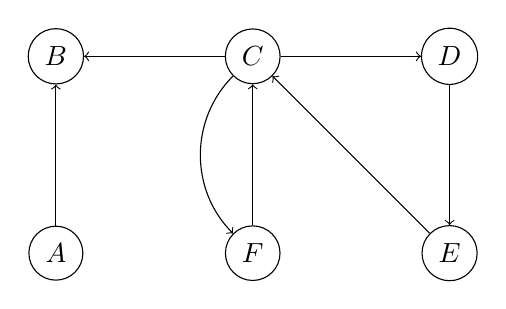
\begin{tikzpicture}[node distance={25mm}, main/.style = {draw, circle}] 
\node[main] (A) {$A$};
\node[main] (B) [above of=A] {$B$}; 
\node[main] (C) [right of=B] {$C$}; 
\node[main] (D) [right of=C] {$D$}; 
\node[main] (E) [below of=D] {$E$};
\node[main] (F) [below of=C] {$F$};

\draw[->] (A) to (B);
\draw[->] (C) to (B);
\draw[->] (C) to (D);
\draw[->] (C) to [out=225,in=135,looseness=1] (F);
\draw[->] (D) to (E);
\draw[->] (E) to (C);
\draw[->] (F) to (C);



\end{tikzpicture} 
\end{center}
\newpage
\section*{Exercise \homeworkNumber.4}

$G = (\set{H,I,J,K,L,M,N},\set{\set{J,M}, \set{H,K}, \set{J,K}, \set{N,K}, \set{M,K}, \set{L,K}, \set{N,M}, \set{L,M}})$

\begin{center}
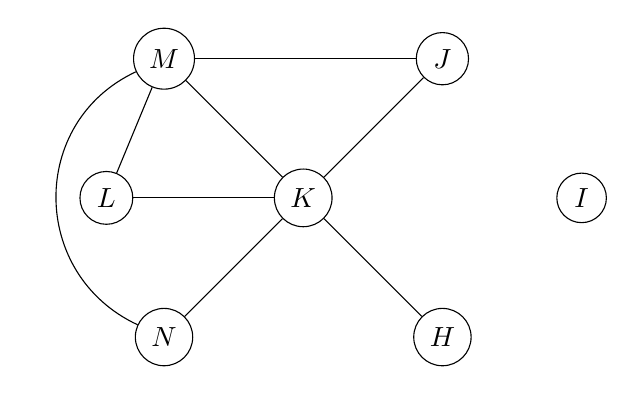
\begin{tikzpicture}[node distance={25mm}, main/.style = {draw, circle}] 

\node[main] (K) {$K$};
\node[main] (H) [below right of=K]{$H$};
\node[main] (J) [above right of=K] {$J$}; 
\node[main] (L) [left of=K] {$L$};
\node[main] (M) [above left of=K] {$M$};
\node[main] (N) [below left of=K] {$N$};
\node[main] (I) [below right of=J] {$I$};

\draw (J) to (M);
\draw (H) to (K);
\draw (J) to (K);
\draw (N) to (K);
\draw (M) to (K);
\draw (L) to (K);
\draw (N) to [out=155,in=205,looseness=1.2] (M);
\draw (L) to (M);

\end{tikzpicture} 
\end{center}

\section*{Exercise \homeworkNumber.5}

\begin{enumerate}[a)]
\item $\langle D, B, C, B, A, B \rangle$

\item $\langle A, B, C \rangle$ \\ 
$\langle C, B, A \rangle$ \\
$\langle D, B, A \rangle$ \\
$\langle D, B, C \rangle$

\item $\langle A, B, C, B, A \rangle$

\item zero


\end{enumerate}





\end{document}
